% !TEX root = ../MemPod.tex

\section{Predicting Hot Regions}
\label{sec:MEA}

%Memory management mechanisms need the ability to monitor and profile accesses to memory in order to identify hot regions and migrate them. Traditionally, a full set of counters is used, with one counter per physical page -- or region depending on the mechanism's granularity -- in order to accurately keep count of all accesses to all regions. Periodically these counters must be sorted in order to identify the regions with the highest counts. The identified regions will serve as a ``prediction'' for the next interval (i.e. the hottest page of the current interval will be amongst the hottest pages of the following intervals).

Migration mechanisms predict \textit{future} hot pages to migrate them into fast memory. Prediction accuracy is critical to high performance, as each migration must be amortized by many future accesses to justify the cost of migration.
A commonly used practice is to identify the hot regions within an interval 
and assume that those regions will be hot in the next interval. To accurately identify the hottest regions some mechanisms use an access counter per region. 
At the end of each interval the counters are sorted to identify the highest 
ranked (i.e., most accessed) regions. However, application phase changes could render this approach unsuccessful. Additionally, the number of necessary counters increases linearly as memory capacities grow.

To address the above limitations, we adopt a technique based on the Majority Element Algorithm (MEA). MEA was originally proposed by Karp et al. \cite{karp-mea} and was studied in-depth by Charikar et al. \cite{charikar-mea} for database management and big data analytics. This heuristic has formally been proven to correctly identify the $K$ most frequently occuring elements of a set, when each of those elements appears more than $N \over K+1$ (i.e. has majority), where $N$ is the number of elements in the input set. 

%MemPod uses the ``Majority Element Algorithm'' $(MEA)$ for its activity tracking needs. MEA attempts to identify the \textit{majority} elements in a set. For example in an array with integers, MEA can be used to identify the \textit{K majority numbers}. Majority elements are the most frequently occurring elements, as long as they exist more than $N \over K+1$ times in the information stream (i.e. they have majority), where N is the number of elements in the array.

%The MEA algorithm was originally proposed in \cite{karp-mea} and studied in-depth in \cite{charikar-mea} as a heuristic capable of efficiently identifying majority elements in a stream. This algorithm is formally proven to be 100\% accurate, as long as the K most frequently occurring elements it must identify have majority. With complexity $O(N)$ it could be an ideal candidate for real-time streams of information, such as a stream of memory requests.


%\setlength{\textfloatsep}{5pt}
\begin{algorithm}[t]
%\centering
% \small
 \DontPrintSemicolon
 %\dontprintsemicolon
 \;
 \PrintSemicolon
 %\printsemicolon
 
 \KwIn{X: Set of N elements}
 \KwIn{K: Number of elements to output}
 \KwData{T: Map structure with K entries}
 \KwResult{Set of K majority elements}
 \DontPrintSemicolon
 %\dontprintsemicolon
 \;
 Initialization: $T \leftarrow \emptyset$\; 
 \;
 \PrintSemicolon
 %\printsemicolon
 \ForEach{$i \in X$} {
 	\uIf{$i \in T$}{
		$T[i] \leftarrow T[i] + 1$\;
	}
	\uElseIf{$|T| < K - 1$}{
		$T[i] = 1$\;
	}
	\Else{
		\ForAll{$j \in T$}{
			$T[j] \leftarrow T[j] - 1$\;
			\lIf{$T[j] == 0$}{$T \leftarrow T \setminus {j}$}
		}
	} 
 }
 \caption{Majority Element Algorithm}
 \label{alg:mea}
 
  %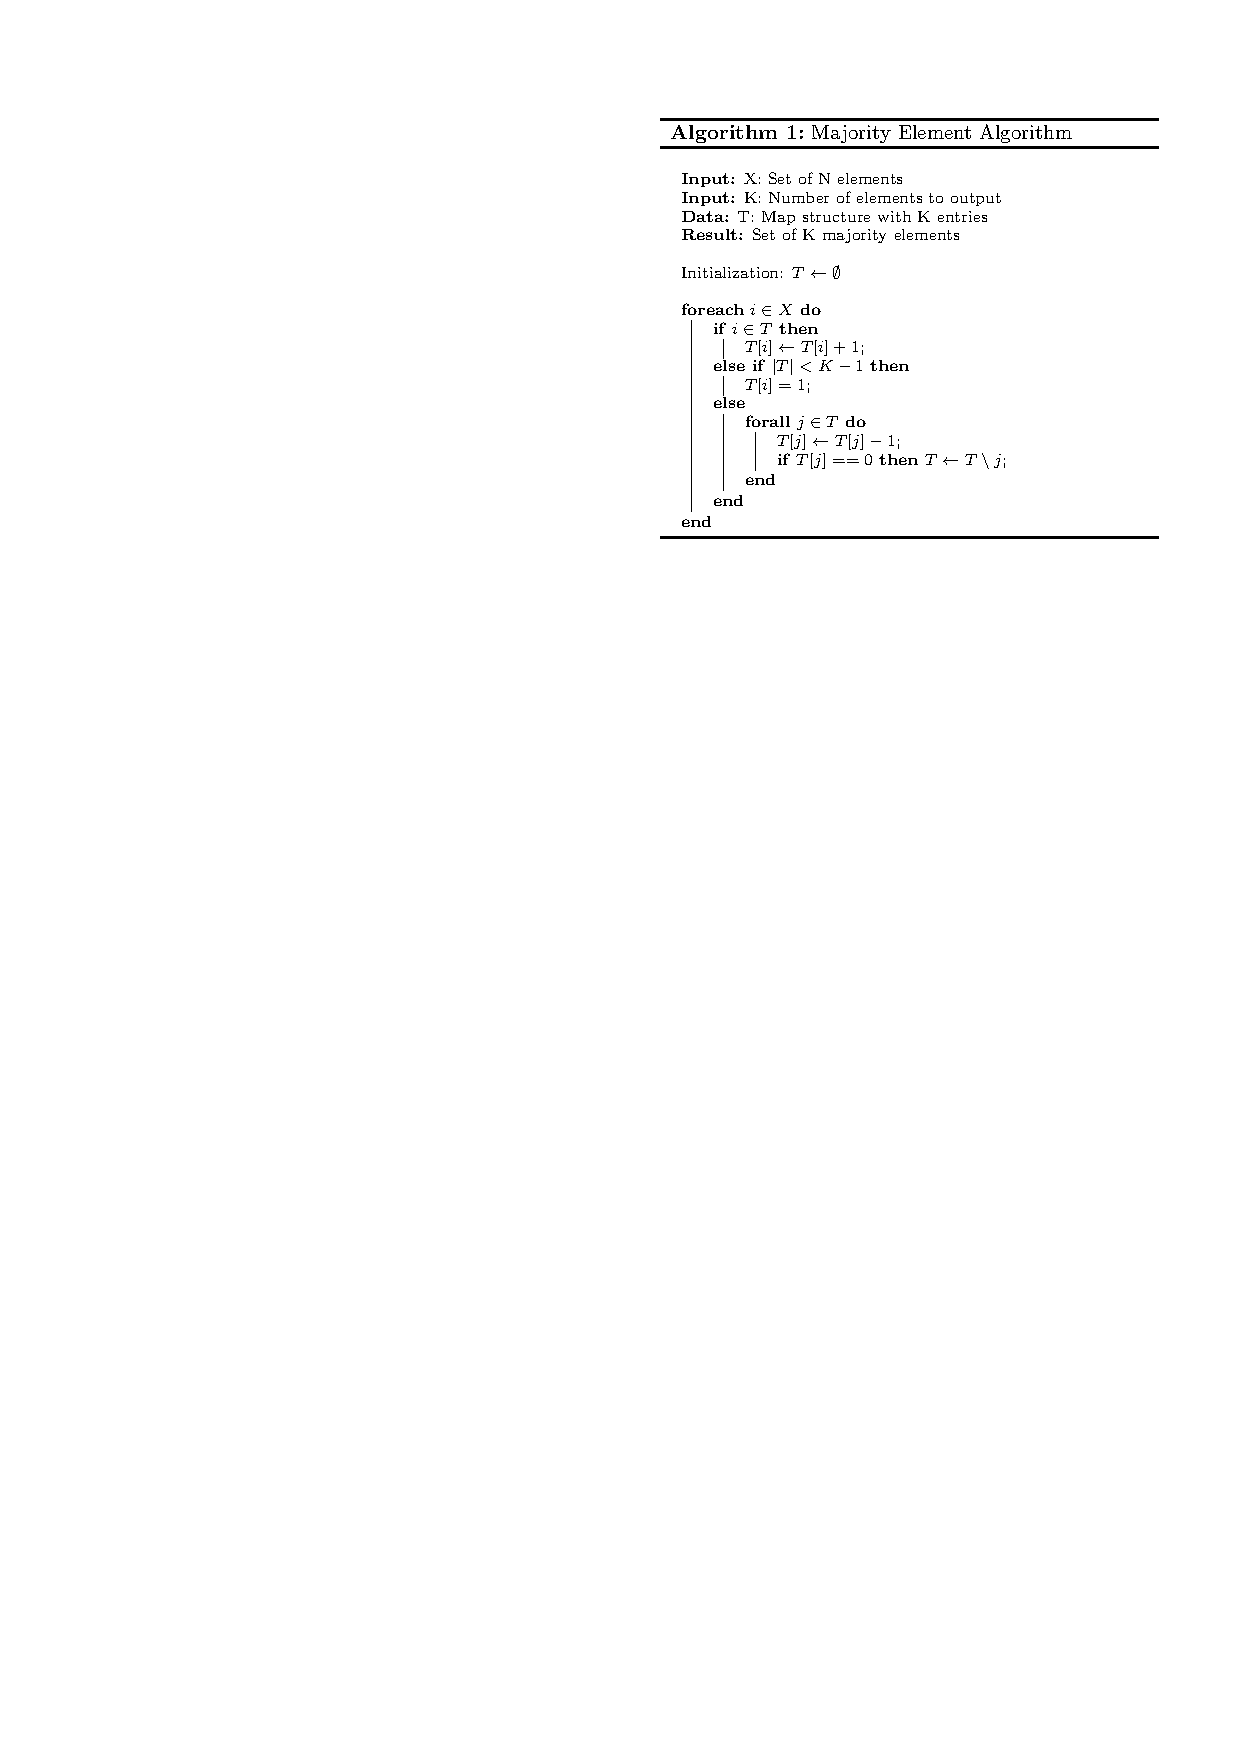
\includegraphics[scale=0.95]{figures/mea_algorithm.pdf}
  
%%%%%%%%% DEAN if you are having issues compiling this on Linux, comment out the algorithm and use the image instead.  
  
  
\end{algorithm}

%\begin{algorithm}
%	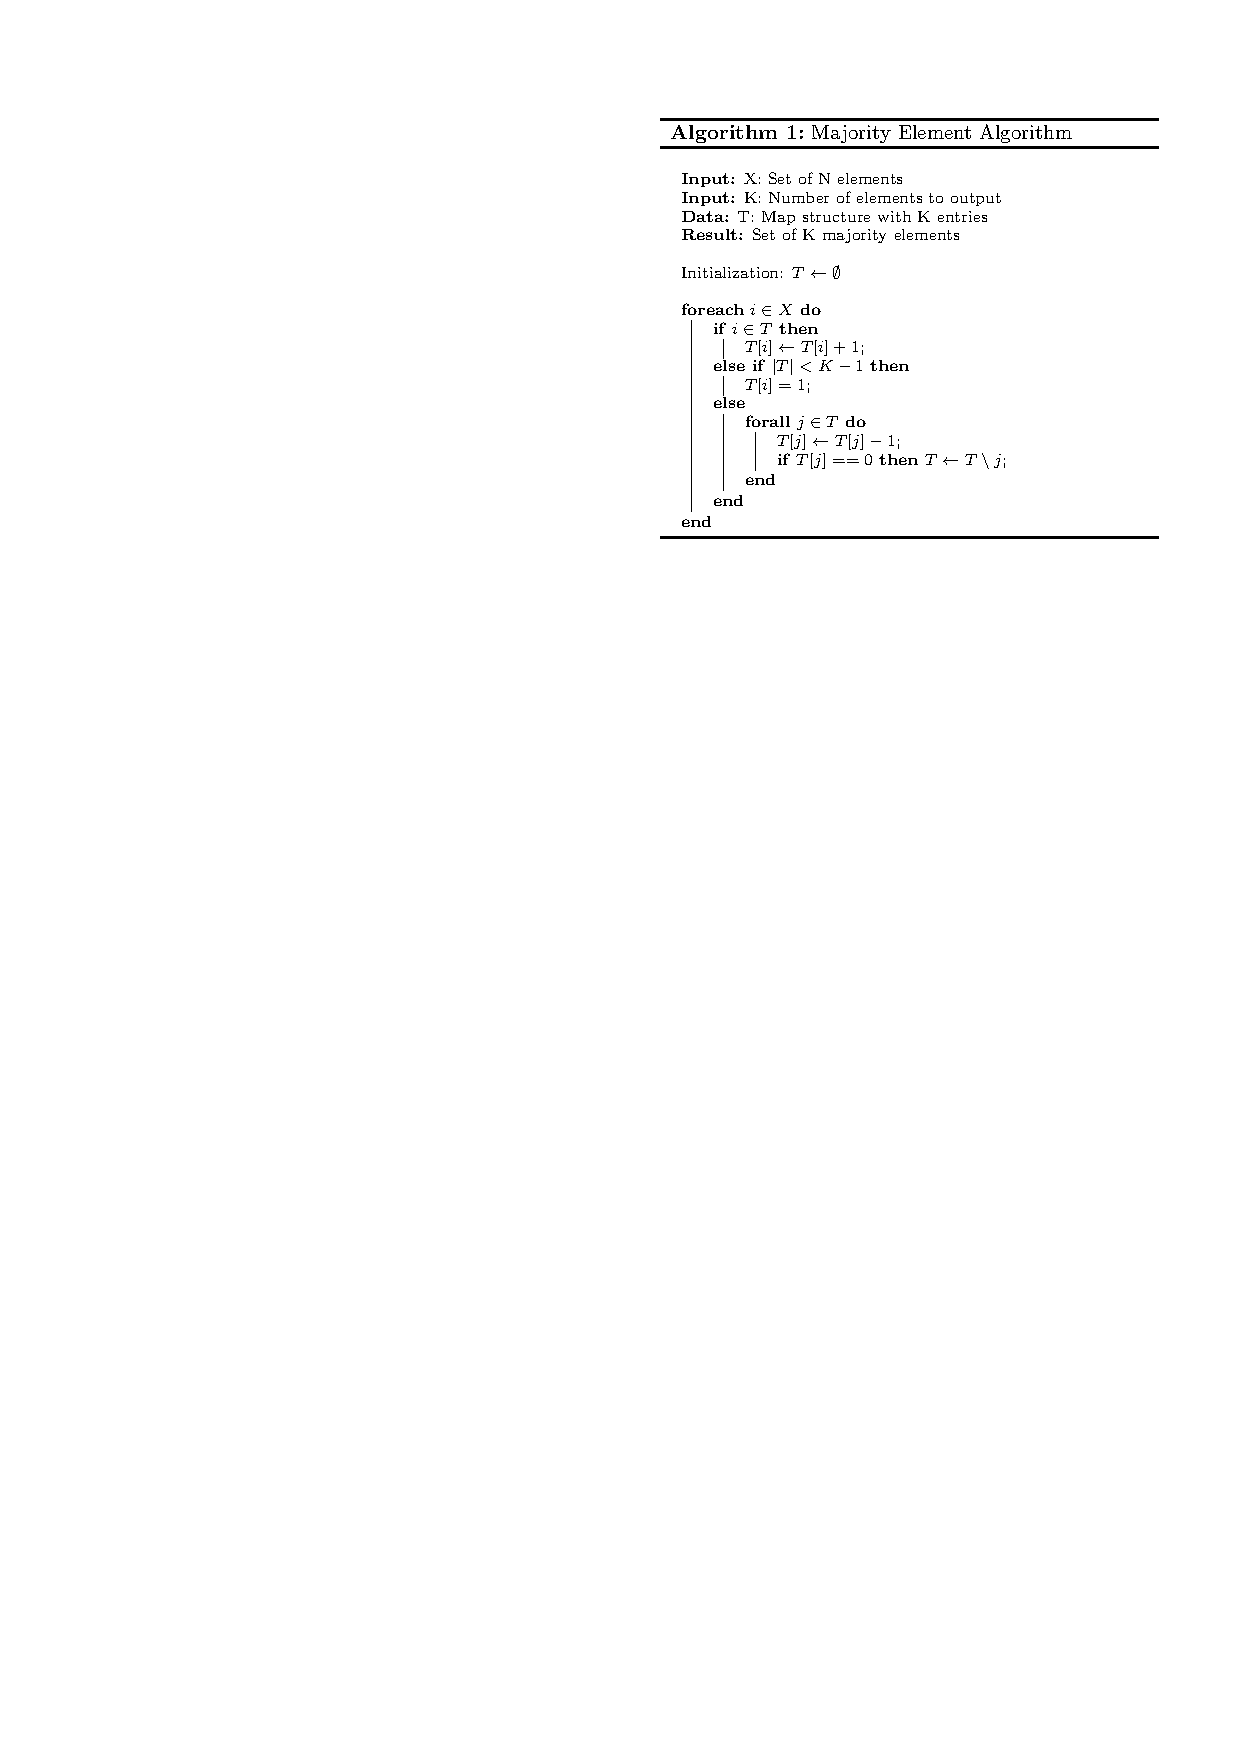
\includegraphics[width=0.45\textwidth]{figures/mea_algorithm.pdf}
%	\caption{TEST}
%	\label{alg:mea}
%\end{algorithm}

MEA is presented in Algorithm \ref{alg:mea} as applied to an array of integers X. A map structure T maps K element IDs (in our integer array example, IDs are the integers' values) to K counters. Looping through the array, if the next integer exists in the map, its counter is incremented by 1. Otherwise, if there's enough room in the map a new entry is added with a count of 1. If the number does not exist in the map and all K counters are occupied, MEA subtracts 1 from every counter, removes the entries with a counter value of 0 and proceeds to the next integer. Once the entire array is processed, the map entries hold the majority elements. 

%Even though this heuristic is 100\% accurate, in the absence of its main assumption no guarantees can be made. The outcome of this algorithm relies on several uncontrolled variables, such as the order our requests appeared in. However, the nature of the algorithm presents a very welcomed side effect: Elements accessed repeatedly can be evicted from the map by elements that were accessed less times but more recently. This observation reveals MEA's favoritism towards temporal locality. Furthermore, the area overhead of this algorithm implemented in hardware remains constant, regardless of how many elements need to be profiled (i.e. regardless of how many pages exist in main memory). 

In our application of MEA to activity tracking, the sequence of page addresses accessed correspond to the array of integers in the above example. 
However, we find that the sequence of accessed pages typically does not
meet the condition of MEA that guarantees it will find the most-accessed
pages; thus, it becomes an approximation.  What makes MEA most useful,
though, is its failure mode -- when it fails to find the most-accessed pages,
it does so by favoring recency over quantity.  That is, a page accessed several
times near the end of an interval can easily knock out a page accessed many
more times early in the interval.  As a result, it combines both access
counting and temporal locality, at a fraction of the cost of access counting
alone.

\remark{Nuwan's comment on next sentence: The "number of regions in memory" isn't really the input set, right? Input set is explained above as the sequence of accesses. Further, it's not entirely true that area overhead is constant with the number of regions. As the region count grows, the size of the map needed to hold those region IDs will grow. Admittedly, it grows as log2(number of regions). So it's very slow growth, but not constant. I won't edit; I'll let you address these points however you see fit.}
\remark{A.P.: I agree that the term input set is wrong here. I updated the text. But I disagree that MEA overhead grows. We could keep it at 128 if we want regardless of the memory size. It's possible that we'll want to use more counters, but the option of keeping it constant is still there}

MEA's area overhead grows slowly with the amount of memory per pod.  The 
number of counters can be kept constant, but the size of the 
ID or tag grows with the log of the memory size.
Its $O(N)$ time 
complexity works well for analyzing a stream of access requests in real time, and eliminates the need for sorting the counters.

%In a memory management scheme that uses Full Counters and a scenario where we want to identify the 100 ``hottest'' pages, we would need one full counter per memory page and on top of that we would have to periodically sort all those counters to pick the top 100. With the use of MEA counters we only need a map with 100 entries regardless of the actual number of pages in main memory. In an 8GB memory with 2kB pages and looking for the top 100 pages, MEA needs $\sim$5K times fewer bits than the full counters' storage requirements (4MB Vs 850B). Considering all the potential benefits MEA can offer in theory, we compared its counting and prediction accuracy against the Full Counters (FC) scheme. 

\subsubsection*{MEA Evaluation}

In this section, we seek to understand the effectiveness of MEA's counting 
and prediction accuracy, compared against a Full Counters (FC) scheme,
independent of the MemPod architecture. We use memory traces captured 
from multi-programmed 8-core workloads (the same traces used and described in Section \ref{sec:Results}) and simulated MEA and FC side-by-side with an in-house off-line simulator that provides oracle knowledge of future intervals. 
\remark{Nuwan's comment on next sentence: What's the significance of 50us here?\\A.P.: At the time, 50us used to be the best interval length for MemPod so I went with it.}

The interval size for both MEA and FC was set at 5500 requests which is the average number of requests serviced within a 50us window in our timing experiments. For this experiment we used 128 MEA counters and FC requires 4.5M counters (assuming a 1+8GB memory capacity). 
We do two comparisons in this study.  First, we examine the ability of MEA
to identify the top pages in the past interval, something the full counter
scheme will do perfectly.  Second, we examine the ability of both schemes
to predict the top pages in the next interval.  In both studies, we will
examine the schemes' ability to identify the 30 most-accessed pages, in
bins of 10 each (1-10, 11-20, and 21-30).

\remark{These results don't make sense without knowing how many MEA
counters you used.\\A.P.: Added in text above.}

Figure \ref{fig:mea_1} shows the counting accuracy of MEA for the 
past interval, which should be compared with FC's perfect accuracy.
In some workloads, MEA identified up to 75\% of the top pages. 
However, on average MEA reports accuracy below 55\% on the top tiers. 
Thus, it is a surprisingly ineffective replacement for accurate counters,
if accurate counting were our priority.  The bias toward recent accesses
has a strong effect on the final value of the MEA counters.

\remark{I find this figure odd -- I'd rather see the results grouped by
benchmark grouping than by tier.\\A.P.: Fixed.}

\begin{figure}[t]
\centering
%  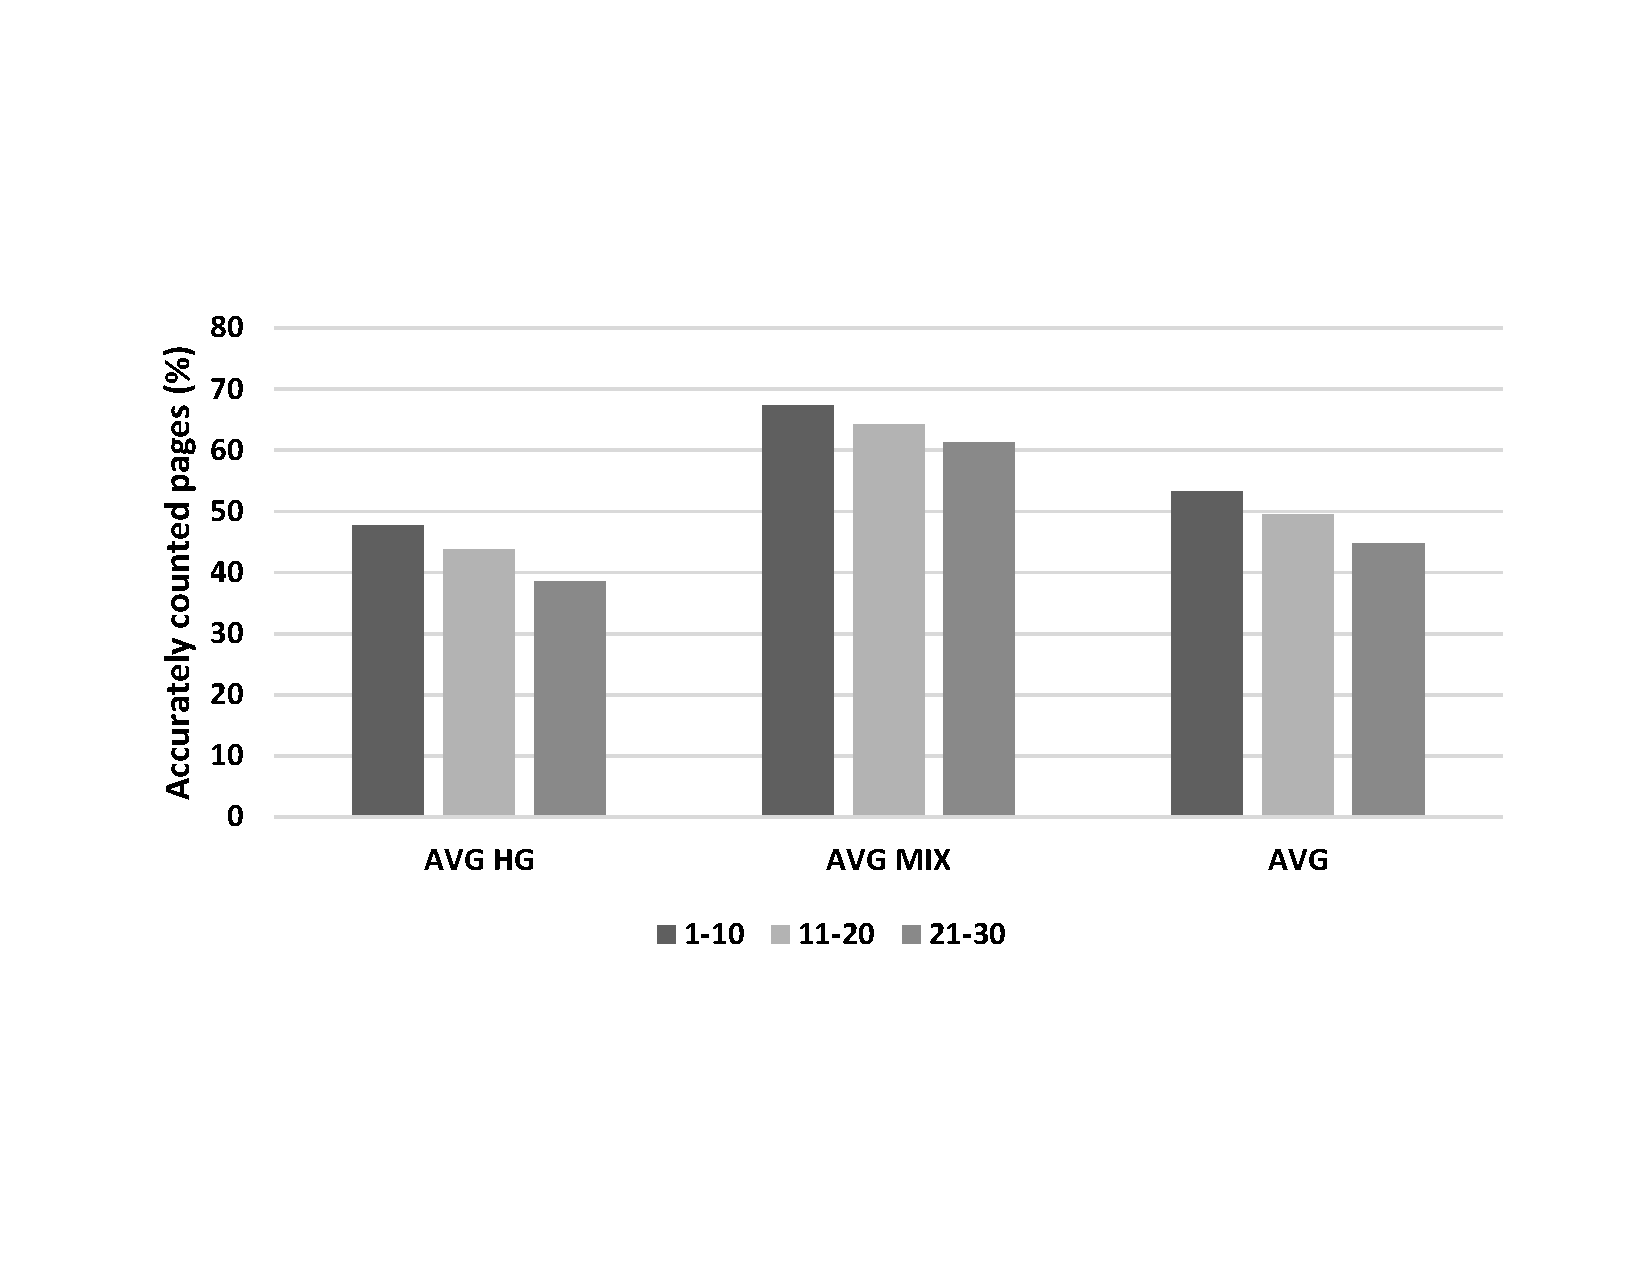
\includegraphics[width=0.46\textwidth, height=9em]{figures/mea_1_v2.pdf}
  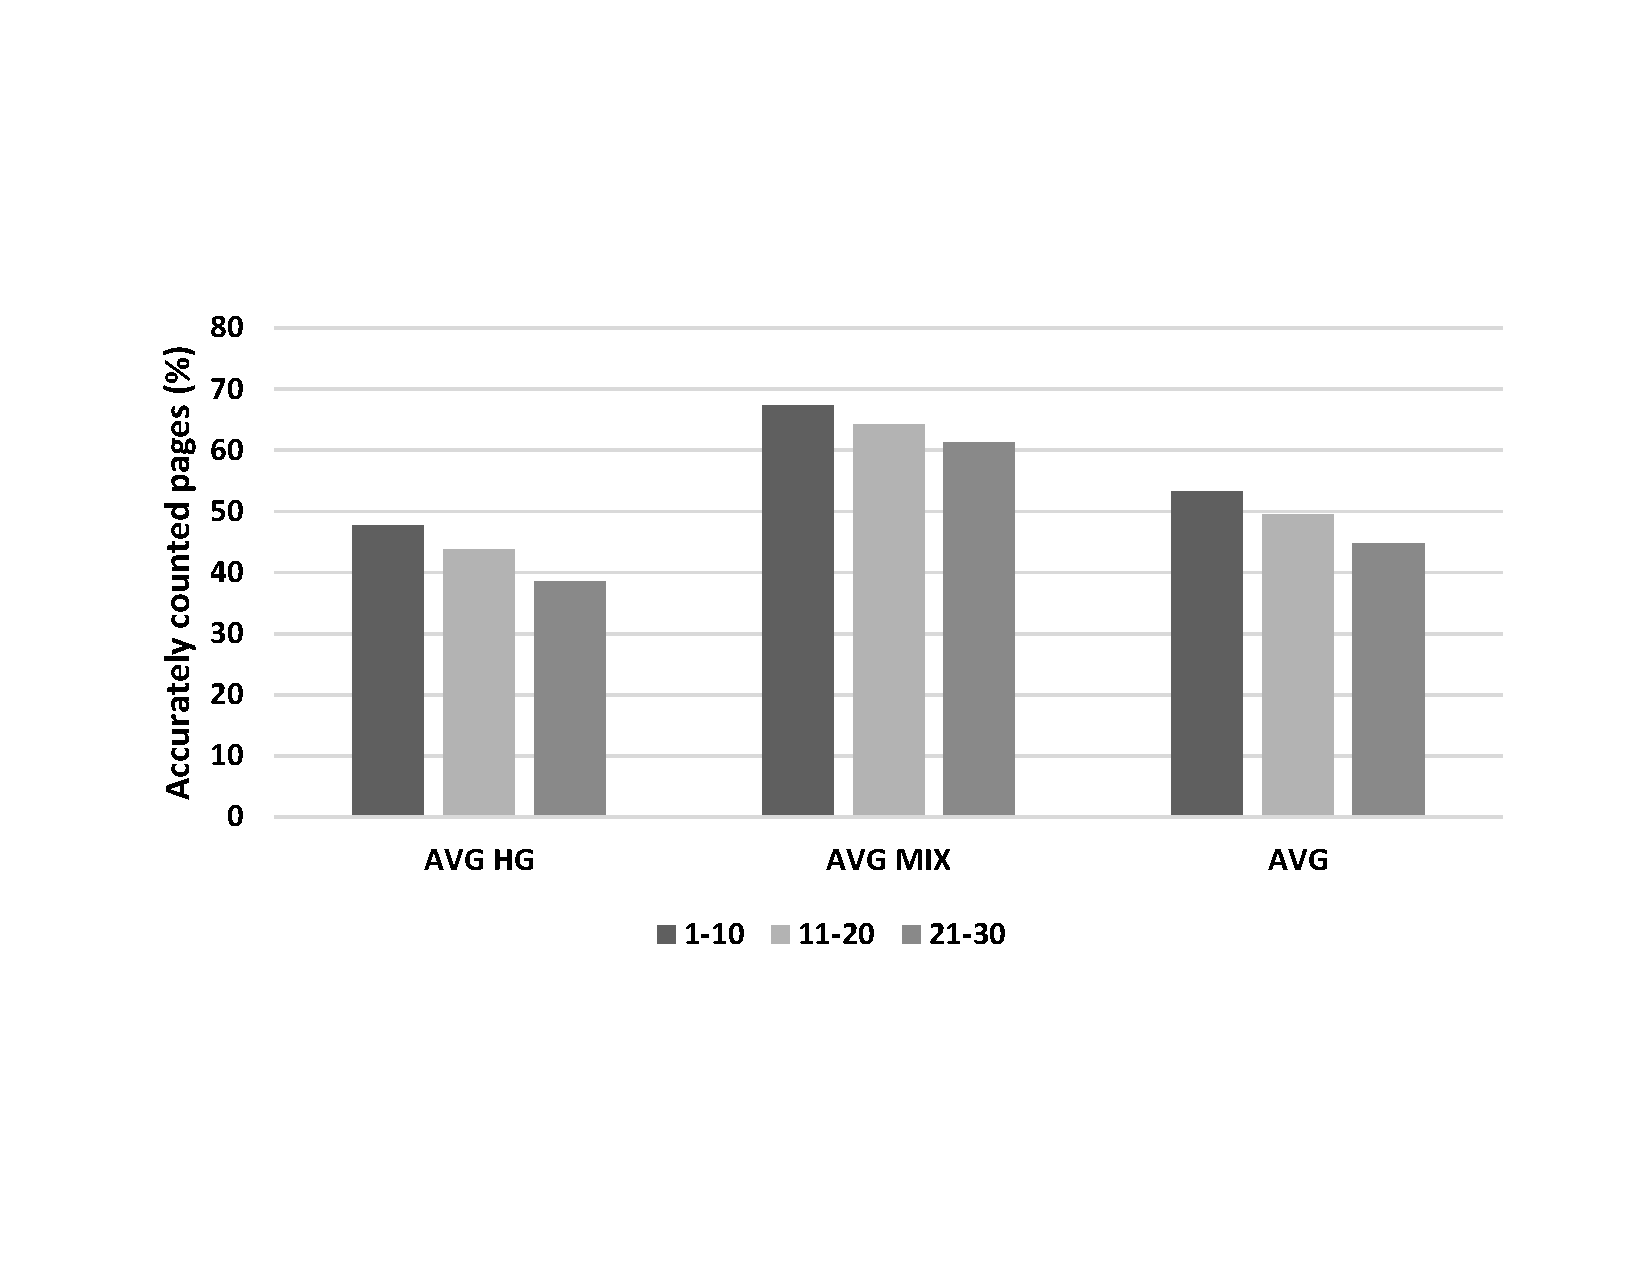
\includegraphics[scale=.3]{figures/mea_1_v2.pdf}
  \caption{MEA counting accuracy compared to Full Counters on the top three tiers (ranks 1-10, 11-20, 21-30). Average results for homogeneous(AVG HG), mixed (AVG MIX) and all (AVG ALL) workloads shown.}
  \label{fig:mea_1}
\end{figure}

When we instead examine the effectiveness in identifying future hot pages,
we see a different story.  Figure \ref{fig:mea_2} presents a comparison of MEA and FC in terms of prediction accuracy. We compare each mechanism's 
``predictions'' against the top three page tiers of the following interval based on oracular knowledge. 
Using 128 counters, MEA will return \textit{up to} 128 predictions based on the past interval, while FC will return an overall ranking of each page accessed. 
In order to be able to directly compare accuracy, 
we take the top N pages from the full counters
each interval,
where N is the number of pages MEA returned.

Figure \ref{fig:mea_2} plots the number of hits on predicted hot pages from the previous interval. We also selected interesting individual benchmarks and show them in Figure \ref{fig:mea_3} to provide a more detailed comparison. 

\remark{Here we're again missing all the critical
details of the experiment.  How many
MEA counters?  How many FC pages were used as ``predictions''?\\A.P.: 128 MEA counters. I used the number of pages MEA returned at each interval as the number of predictions for both mechanisms. Added in text above.}

On average, MEA achieves more future hits than FC by 16\%, 81\% and 68\% on the top three tiers respectively. Figure \ref{fig:mea_3} shows selected individual workloads that generated interesting results and provides a more detailed comparison. Cactus\footnote{We use a single benchmark's name as a shorthand for workloads running the same benchmark 8 times simultaneously on 8 cores.} is the only workload where FC outperformed MEA's prediction. In fact it outperformed MEA on every tier. 

Xalanc and mix9 are most representative of our overall
results. We can see MEA outperforming FC's prediction accuracy in every bin. 
The last two workloads we selected, bwaves and lbm, show FC failing entirely to predict the future (FC also scored zero future hits with our libquantum workload). With bwaves (and libquantum) MEA reports a very low number of future hits but not zero. These results can happen when an application streams through large structures
that exceed the size of the interval.  In that case, the past interval has 
little overlap with the next interval, but recent accesses are much more
likely to be overlapped.
Lbm shows an interesting result, where MEA reports 
a high number of hits (outside of the first tier) in a workload where 
FC failed entirely.  This can happen with a large working set where the 
application does a fairly constant amount of work per page.  Full counters,
then, will record the highest access counts for pages the application is done
with, while MEA will favor pages the application was still working on at the
end of the interval.

\begin{figure}[t]
\centering
  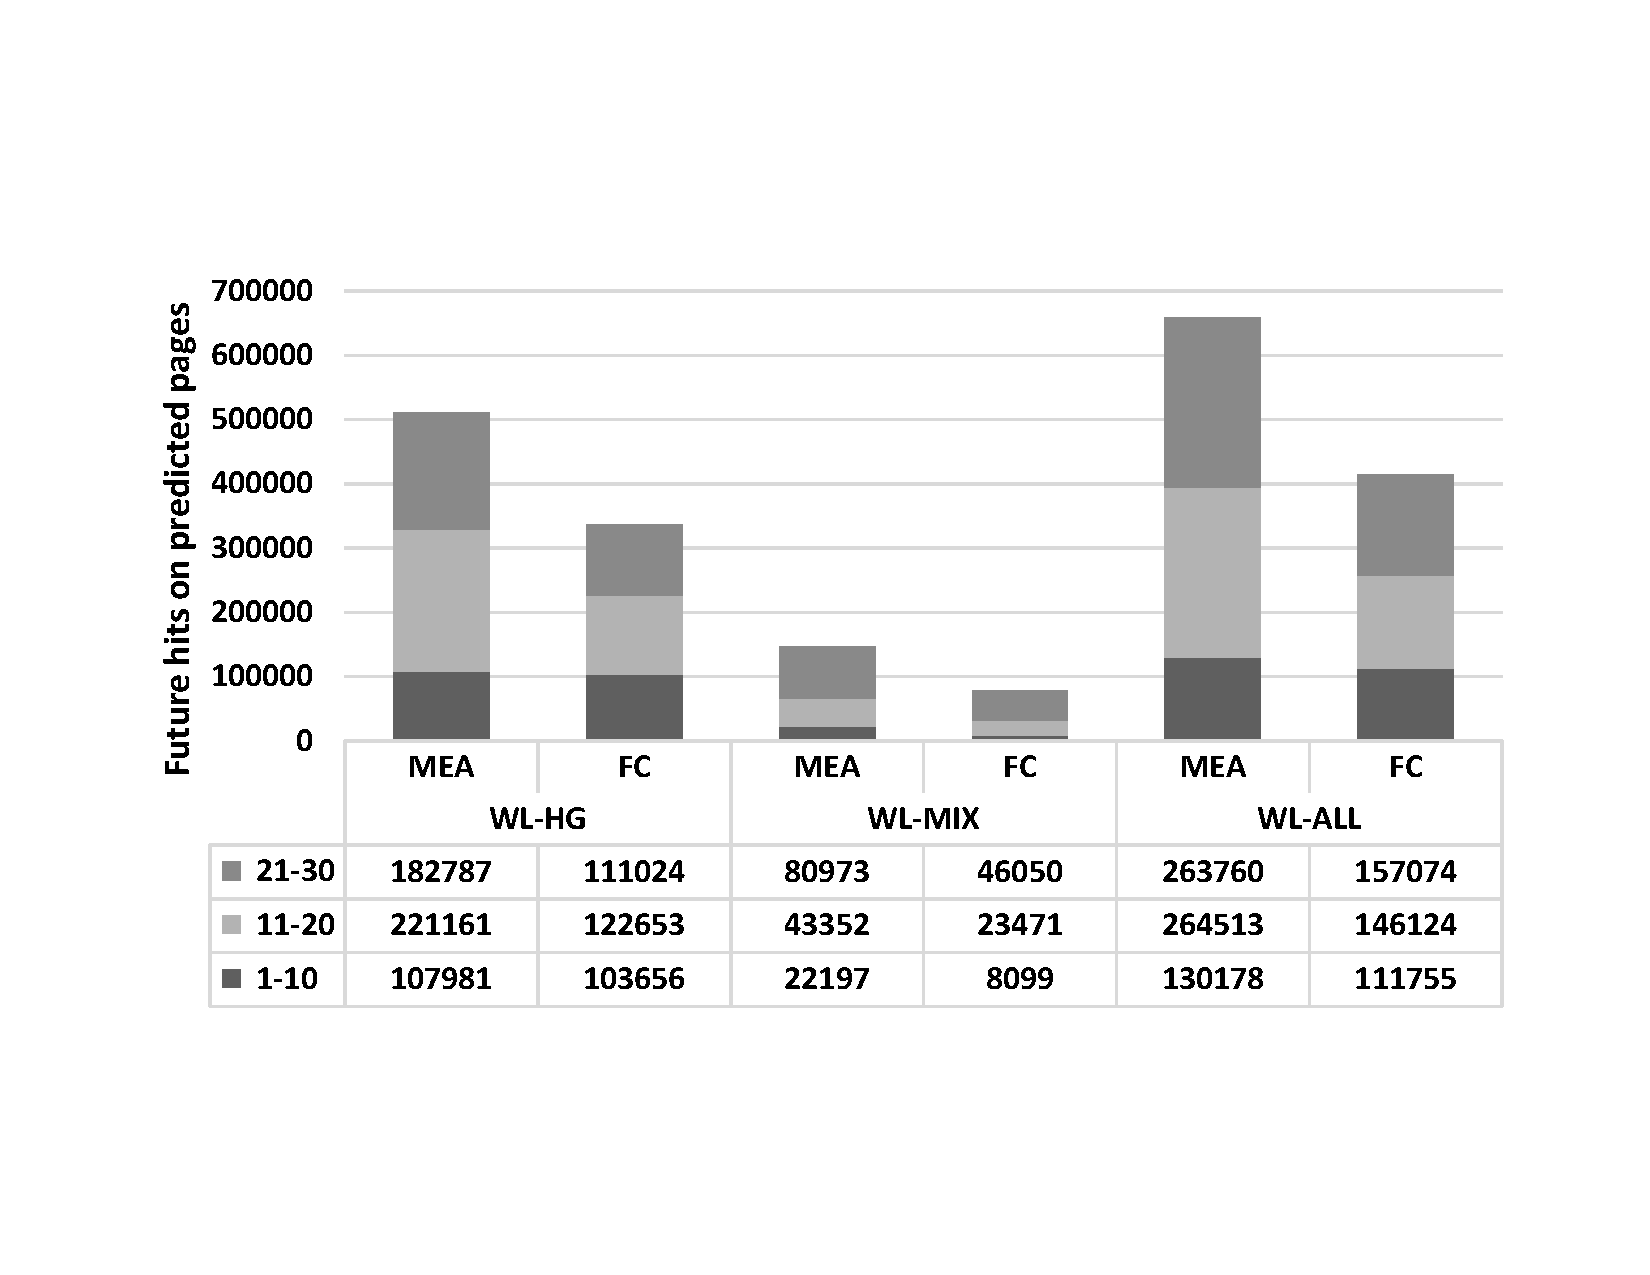
\includegraphics[scale=.3]{figures/mea_2_v2.pdf}
  \caption{MEA prediction accuracy (part 1) compared to Full Counters on the top three tiers (ranks 1-10, 11-20, 21-30). Results for homogeneous(WL-HG), mixed (WL-MIX) and all (WL-ALL) workloads shown.}
  \label{fig:mea_2}
\end{figure}

\begin{figure}[t]
\centering
  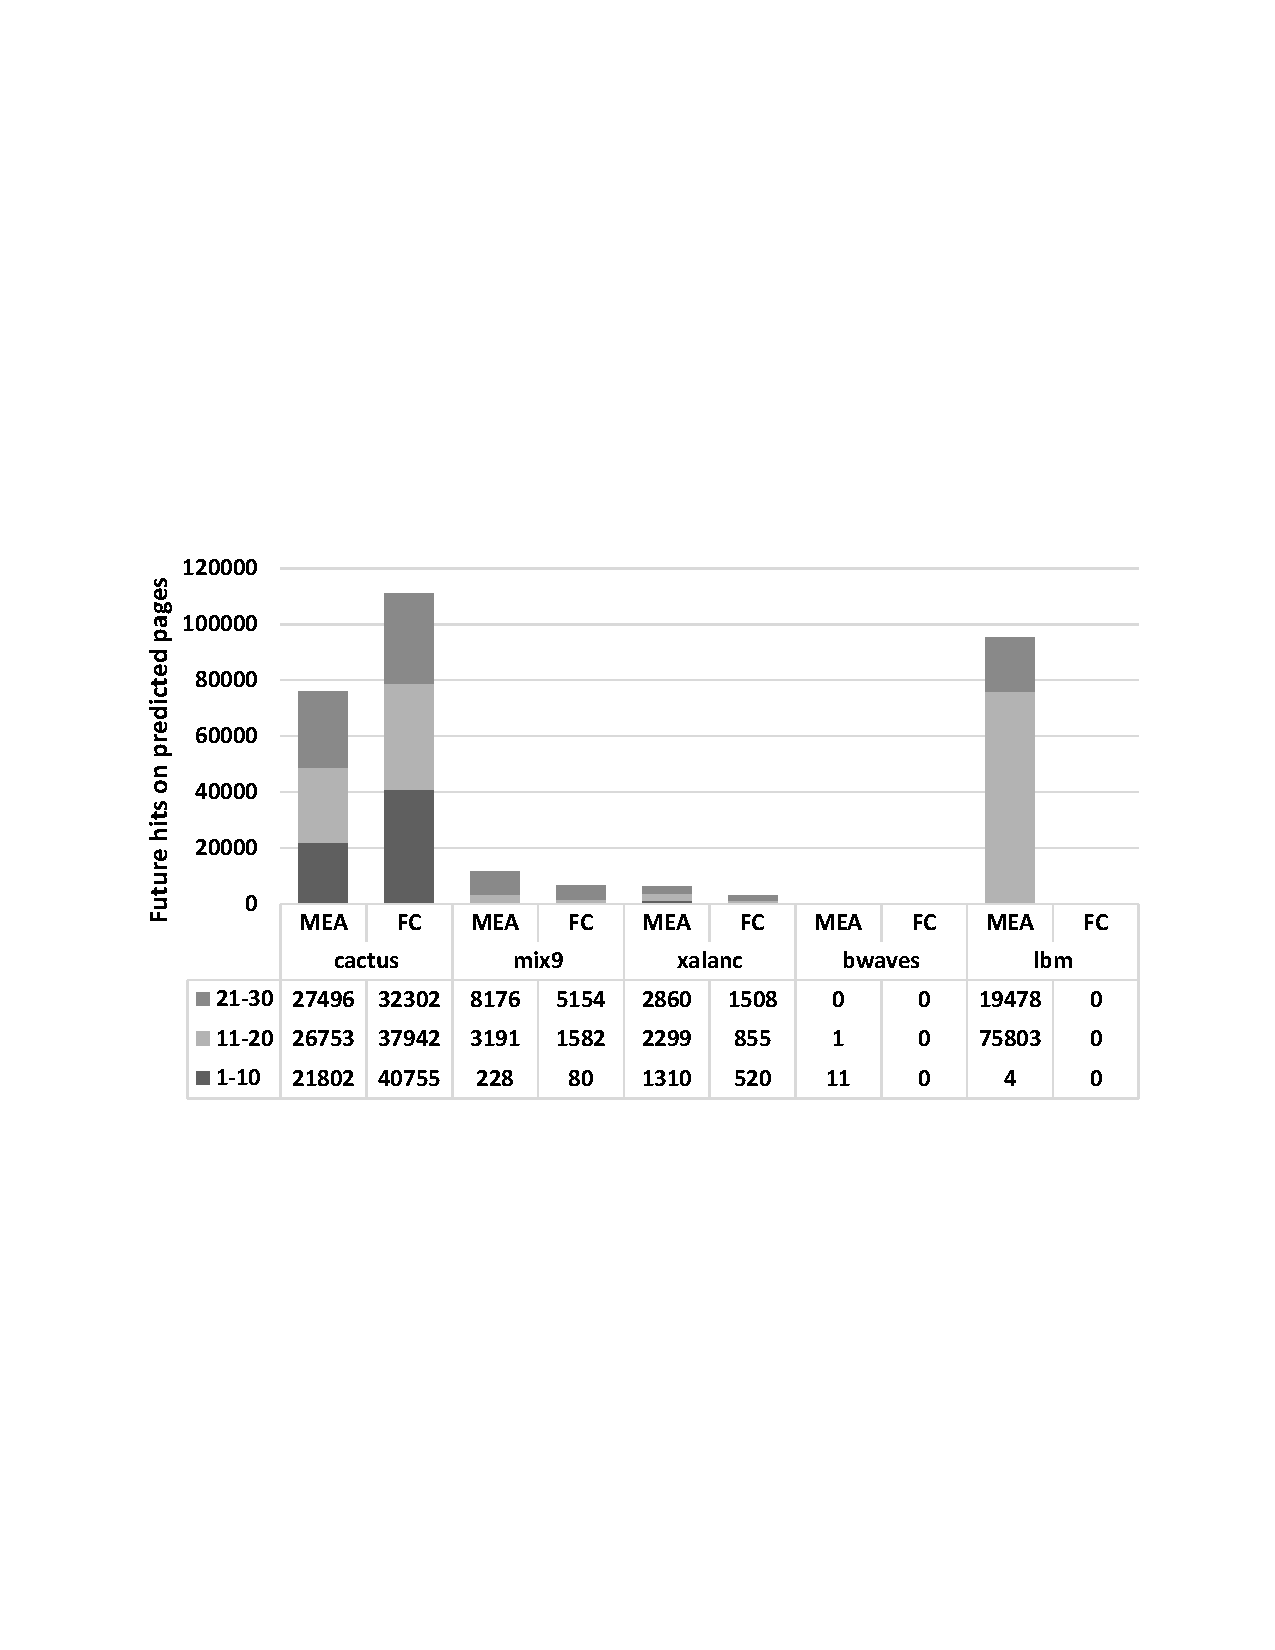
\includegraphics[scale=.45]{figures/mea_3_v2.pdf}
  \caption{MEA prediction accuracy (part 2). This graph presents the most interesting results from individual workloads.}
  \label{fig:mea_3}
\end{figure}

MEA has not previously been used in any kind of architectural event
tracking; however, our results indicate it is an attractive
alternative to full counters at a very small fraction of the hardware cost.
